\documentclass[12pt]{article}
\usepackage{listings}
\usepackage[colorlinks=true,pagebackref,linkcolor=blue]{hyperref}
\textwidth=7in
\textheight=9.5in
\topmargin=-1in
\headheight=0in
\headsep=.5in
\hoffset  -.85in

\lstset{
basicstyle=\footnotesize\ttfamily,
language=bash,
upquote=true,
breakatwhitespace=true,
columns=fullflexible,
keepspaces,
%numbers=none,
tabsize=3,
frame=blrt,
framextopmargin=5pt,
showstringspaces=false,
extendedchars=true
}

\pagestyle{empty}

\renewcommand{\thefootnote}{\fnsymbol{footnote}}
\usepackage{graphicx}
\begin{document}



\begin{center}
{\bf AMS 550.400 \quad HW SET 1\quad  Due Date:  Oct 8}\\
\vskip.2in
{\footnotesize Last Compiled on \today}
\end{center}

\setlength{\unitlength}{1in}

\begin{picture}(6,.1) 
\put(0,0) {\line(1,0){6.25}}         
\end{picture}

 

\renewcommand{\arraystretch}{2}

\vskip.25in
\noindent\textbf{Problem 1 (10 pts):}  

\vskip.25in
\begin{enumerate}
\item mkdir hw1p1.git 
\item cd hw1p1.git 
\item git init . 
\item vi main.txt
\item git add .
\item git commit -m "A added to master"
\item vi main.txt
\item git add .
\item git commit -m "B added to master branch"
\item git branch alt
\item git branch
\item vi main.txt
\item git add .
\item git commit -m "C added to master branch"
\item git checkout alt
\item vi main.txt
\item git add .
\item git commit -m "X added to alt branch"
\item git checkout master
\item git merge alt
\item vi main.txt
\item git add .
\item git commit -m "Alt merged to master branch"
\item git branch
\item vi main.txt
\item git add .
\item git commit -m "D added to master branch"
\item git log --graph --oneline
\item git checkout alt
\item git log --graph --oneline
\end{enumerate}

\begin{figure}[h]
    \begin{center}
        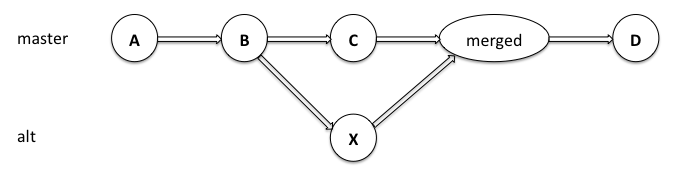
\includegraphics[width=\textwidth]{master_commitgraph.png}
    \end{center}
    \caption{Master Commit Graph}
    \label{fig:mcg}
\end{figure}

\begin{figure}[h]
    \begin{center}
        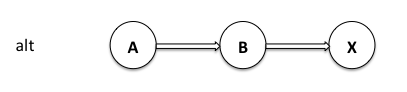
\includegraphics[width=\textwidth]{alt_commitgraph.png}
    \end{center}
    \caption{Alt Commit Graph}
    \label{fig:acg}
\end{figure}

\begin{picture}(6,.1) 
\put(0,0) {\line(1,0){6.25}}         
\end{picture}

\vskip.25in
\noindent\textbf{Problem 2 (10 pts):}

\vskip.25in
\begin{enumerate}
\item mkdir hw1p2.git
\item cd hw1p2.git
\item git init .
\item git remote add s1 git://github.com/nhlee/550400.stanza1.git
\item git pull s1 master
\item vi main.txt
\item git add .
\item git commit -m "Title added"
\item git remote add s2 git://github.com/nhlee/550400.stanza2.git
\item git pull s2 master
\item vi main.txt
\item git add .
\item git commit -m "2nd stanza merged"
\item git remote add s3 git://github.com/nhlee/550400.stanza3.git
\item git pull s3 master
\item vi main.txt
\item git add .
\item git commit -m "3rd stanza merged"
\item git remote add origin https://github.com/tangdnn/550400.homeworkset.1.git
\item git push origin master
\item git remote rm origin
\end{enumerate}

\begin{picture}(6,.1) 
\put(0,0) {\line(1,0){6.25}}         
\end{picture}

\vskip.25in
\noindent\textbf{Problem 3 (40 pts):}

\vskip.25in
For this exercise, we wish to build a cooperative strategy for a team of four students who have split up the presentation into four parts. 
\vskip.15in
\noindent\textbf{Strategy 1:}
\begin{itemize}
\item \textbf{Formulate the Problem.} Since they do not wish to work concurrently, we must develop two different work flow strategies for the team to merge all four parts together without the need for a group meeting using \texttt{git}. 
\item \textbf{Outline the Model.} One work flow strategy for this team is to for the team members to merge their presentation consecutively; i.e.: \emph{B} merge with \emph{A}, then \emph{B} merge with \emph{C}, and lastly, \emph{D} merge with \emph{C}. The endogenous variable of this model is for all four team members to combine their respective parts of the presentation without working concurrently during a group meeting. The exogenous variable of this model is an effective work flow strategy proposal---in this case, merging each part consecutively using \texttt{git}---to combine different parts of the presentation. Unimportant variables that can be neglected are the amount of time it takes to write each part on its own (assuming that at least two parts are done at the time of merging), the physical quantity of each part, and the consistency of each students' writing.
\item \textbf{Is It Useful?}
\item \textbf{Test the Model.}
\item \textbf{Strengths and Weaknesses.}
\end{itemize}

\vskip.25in
\noindent\textbf{Strategy 2:}
\begin{itemize}
\item \textbf{Formulate the Problem.} 
\item \textbf{Outline the Model.} 
\item \textbf{Is It Useful?}
\item \textbf{Test the Model.}
\item \textbf{Strengths and Weaknesses.}
\end{itemize}

\vskip.25in
\noindent\textbf{Final recommendation:}

\begin{picture}(6,.1) 
\put(0,0) {\line(1,0){6.25}}         
\end{picture}

\vskip.25in
\noindent\textbf{Problem 4 (aka.\ Fair Play, 40 pts):}
Answer the following question:
\begin{verse}
Is the tennis game fair?
\end{verse}
Note that unlike Problem 3, this question is vaguely stated.
This is intensional, whence to begin, you will first need to clarify
what exactly your question is.
You may use the class discussion on this particular 
problem, but you \emph{may not} directly refer to our 
discussion.  Instead, formulate the model carefully but concisely in 
your own words.   


\end{document}
